% flashcards-title: Fourths on a number line
% flashcards-desc: A number line from zero to two is divided into fourths, with A at three fourths and B at five fourths.
\documentclass[dvisvgm,tikz,border=8pt]{standalone}
\usetikzlibrary{arrows.meta,patterns}

\definecolor{qraNavy}{HTML}{17324D}
\definecolor{qraBlue}{HTML}{2B6CB0}
\definecolor{qraGold}{HTML}{B7791F}
\definecolor{qraPale}{HTML}{EAF2F8}
\definecolor{qraGray}{HTML}{5C6773}

\tikzset{
  qra axis/.style={draw=qraNavy, line width=1.2pt},
  qra tick/.style={draw=qraNavy, line width=1pt},
  qra guide/.style={draw=qraGray, densely dashed, line width=0.8pt},
  qra counter/.style={circle, draw=qraNavy, fill=qraPale, line width=0.9pt, minimum size=7mm, inner sep=0pt},
  qra label/.style={font=\sffamily\bfseries, text=qraNavy},
  qra small label/.style={font=\sffamily, text=qraNavy},
}

\begin{document}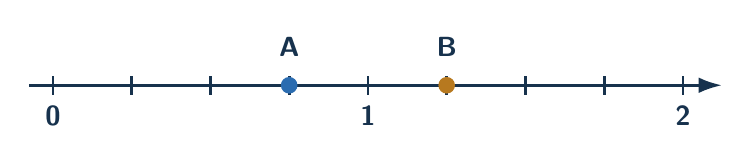
\begin{tikzpicture}[x=1cm,y=1cm]
\draw[qra axis,-{Latex[length=3mm,width=2mm]}](-.3,0)--(8.5,0);
\foreach \x in {0,...,8}{\draw[qra tick](\x,-.12)--(\x,.12);}
\node[qra label,below=4pt]at(0,0){0};\node[qra label,below=4pt]at(4,0){1};\node[qra label,below=4pt]at(8,0){2};
\fill[qraBlue](3,0)circle(3pt);\node[qra label,above=7pt]at(3,0){A};
\fill[qraGold](5,0)circle(3pt);\node[qra label,above=7pt]at(5,0){B};
\end{tikzpicture}\end{document}
